Selon le fait \ref{nece-cond}, si parmi les \ngones\ de périmètre fixé, il en existe un qui maximise l'aire, alors ce ne peut être que le \ngone\ régulier. Nous allons établir que cette condition nécessaire est suffisante. Pour cela, nous avons juste besoin de savoir qu'il existe au moins un \ngone\ d'aire maximale.
Comme dans la remarque \ref{tri-topo-comp}, nous allons convier le couple continuité/compacité, mais ici les choses se compliquent, car nous allons devoir accepter de travailler avec des polygones croisés, et par conséquent il nous faut un moyen de mesurer la surface de tels polygones (le vrai point délicat est ici). 
Pour arriver à nos fins, commençons par expliquer comment \geogebra\ obtient une aire de \num{6.5} pour le polygone croisé ci-après.


\begin{center}
	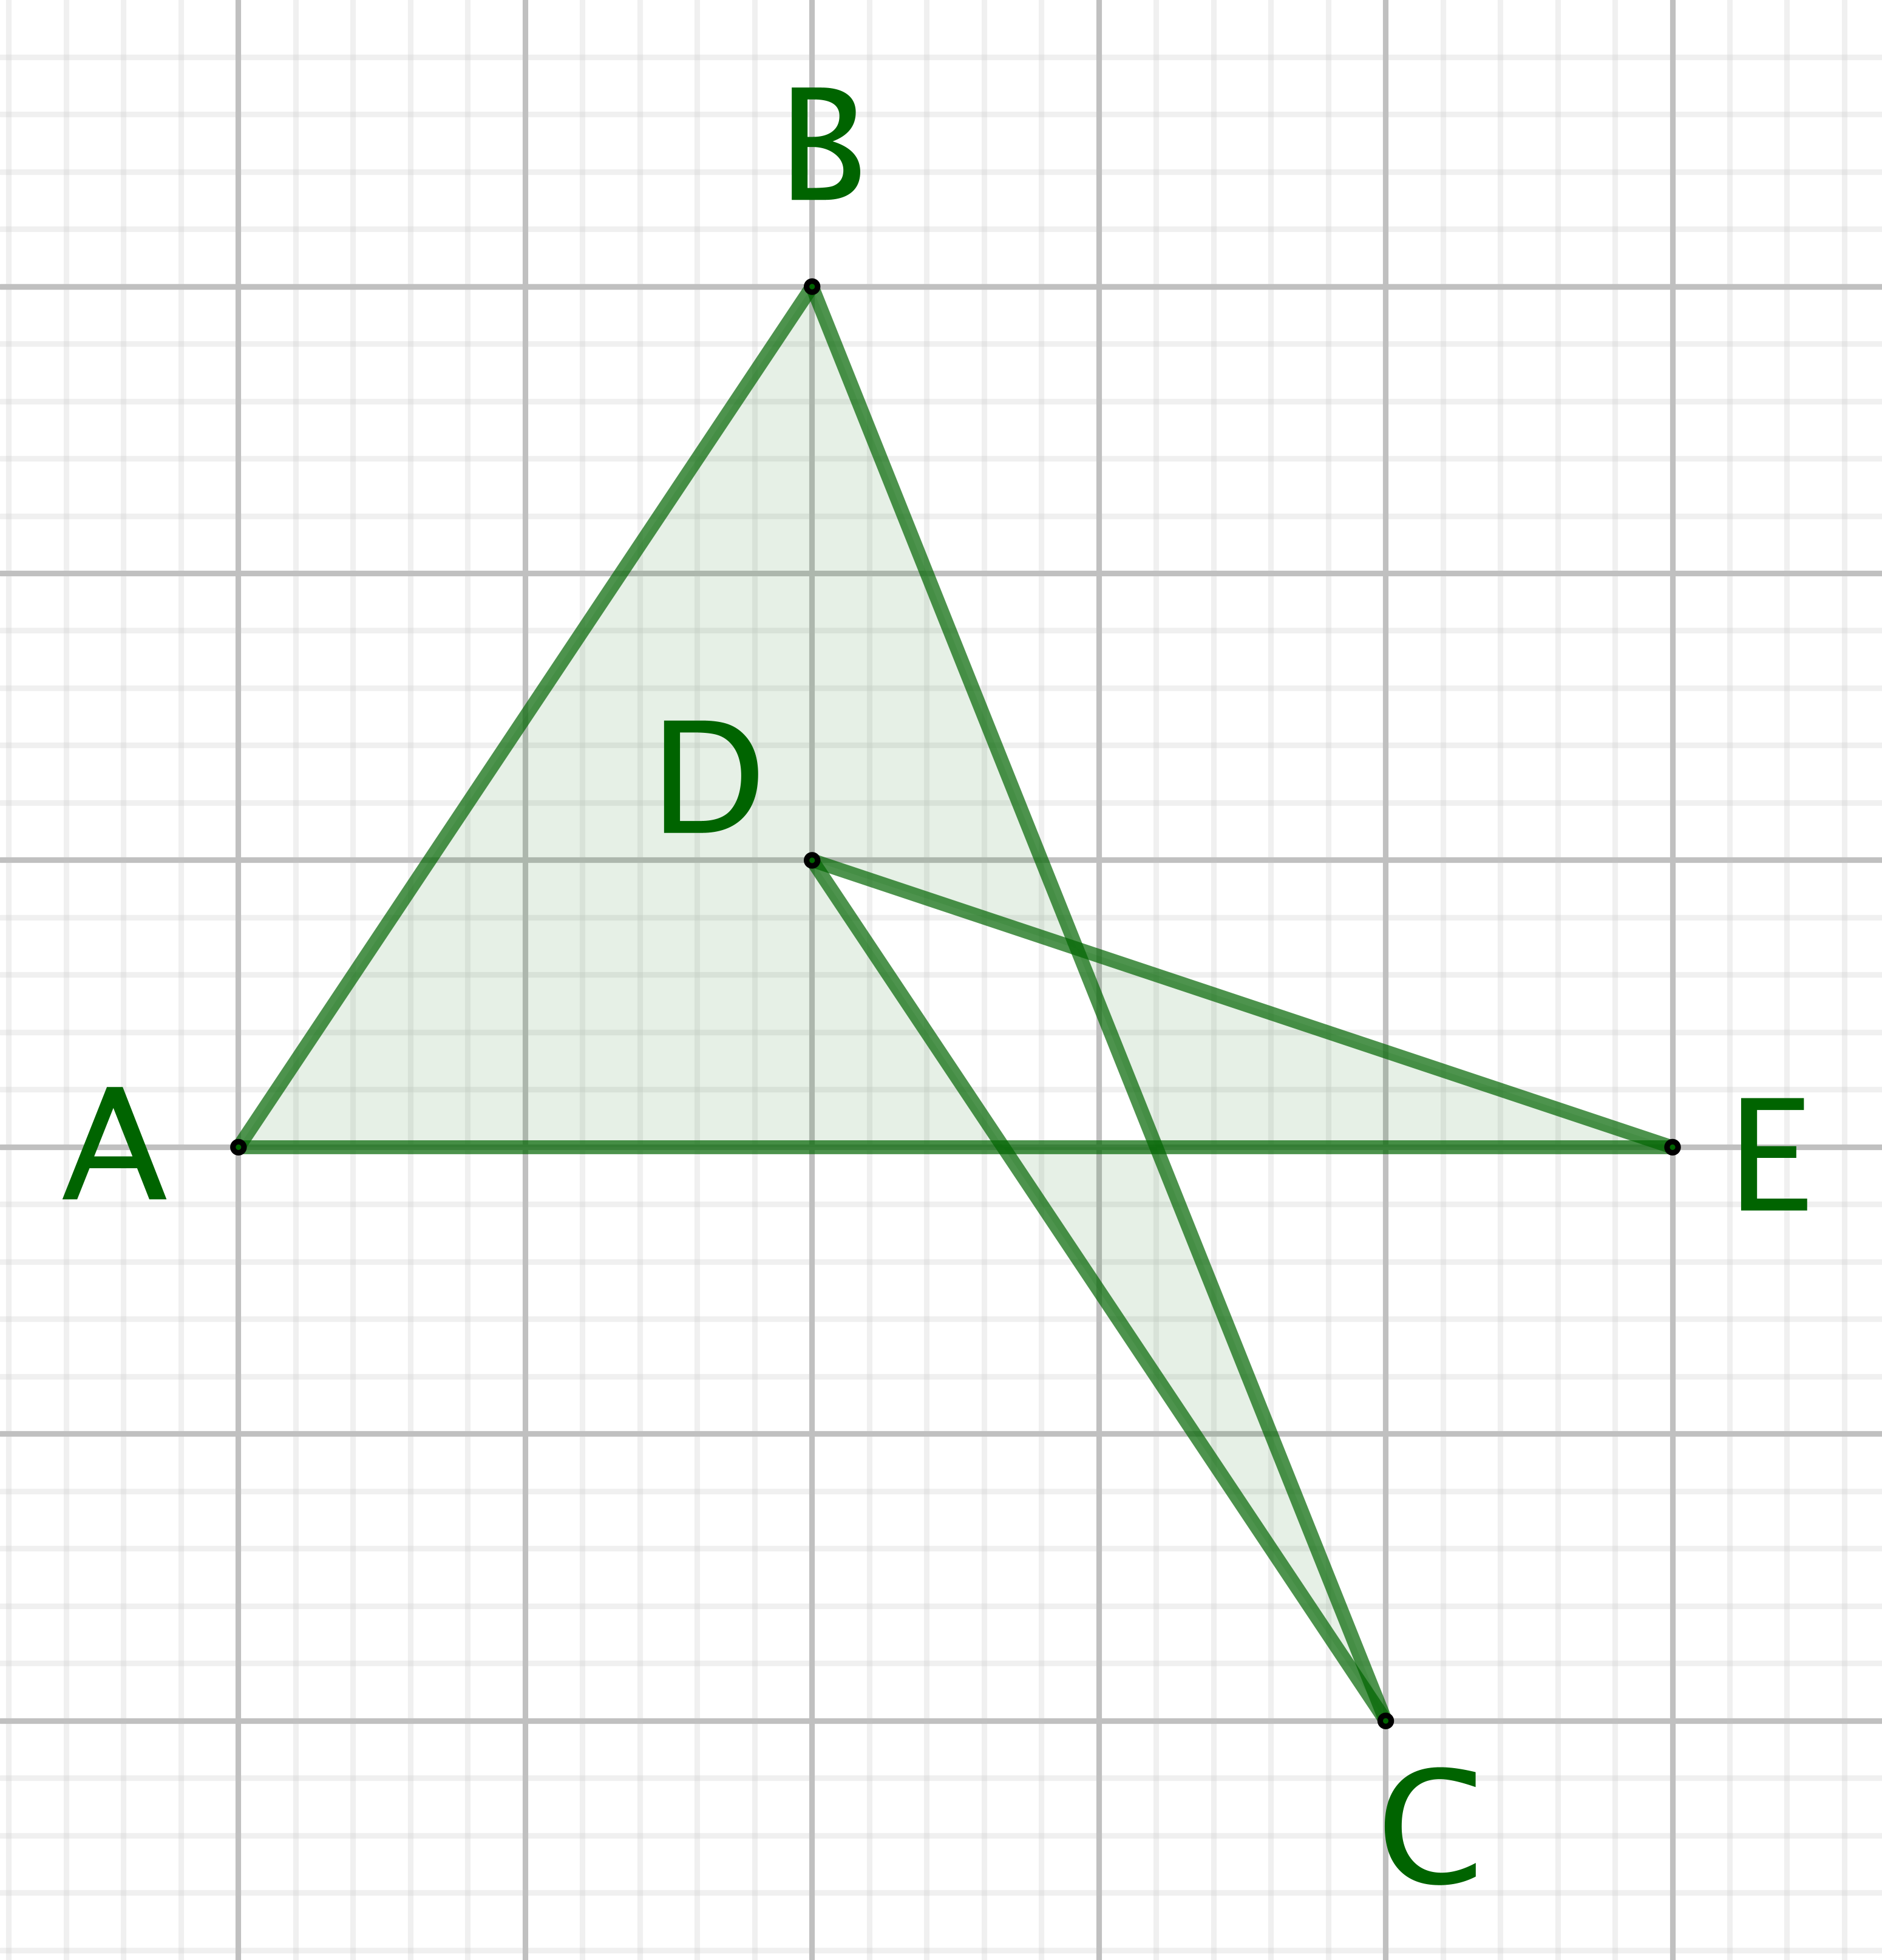
\includegraphics[scale=.4]{content/polygon/sufficient-cond/alg-surf-why.png}
\end{center}


\medskip
%\newpage 
 

L'idée consiste à fixer un point $\Omega$, puis à calculer, via la notion de déterminant, les aires algébriques des triangles indiqués ci-dessous : les aires vertes sont positives, et les rouges négatives (les triangles sont construits en respectant un ordre de parcours des sommets du polygone, et leur orientation est obtenue via le sens anti-horaire comme sens positif).%
\footnote{
	En considérant $EDCBA$ au lieu de $ABCDE$ dans la méthode indiquée, on obtiendrait $(\num{-6.5})$. Pour obtenir une mesure, il faudra prendre la valeur absolue de la somme des aires algébriques des triangles.
}

\begin{multicols}{3}
	\small\itshape
	
	\begin{center}
		\foreach \i in {1,...,5} {
			\smallskip
		
			\includegraphics[scale=.4]{content/polygon/sufficient-cond/alg-surf-why-step-\i.png}
		
			\smallskip
				Étape \i.
		}
	\end{center}
	
	\smallskip
	
	$2 + 10 - 6 + \num{5.5} - 5 = \num{6.5}$
	redonne bien la valeur fournie par \geogebra.
	Le fait suivant explique le bien fondé de cette méthode qui, a priori, pourrait dépendre du point $\Omega$.
	Comme, pour les polygones convexes, on retombera sur leur aire géométrique à un signe près, cette aire algébrique va nous être utile.
	
	\vfill\null
\end{multicols}


Cette notion d'aire algébrique est à manier avec prudence lorsqu'on la découvre. 
Si c'est votre cas, que pensez-vous de l'aire algébrique du quadrilatère croisé $ABCD$ ci-dessous qui est un antiparallélogramme très particulier? Réponse en note de bas de page.%
\footnote{
	La réponse est $0$. Comme nous verrons que le choix de $\Omega$ est libre, il suffit de faire les calculs avec $\Omega$ l'intersection des segments $[AD]$ et $[BC]$.
}

\begin{center}
	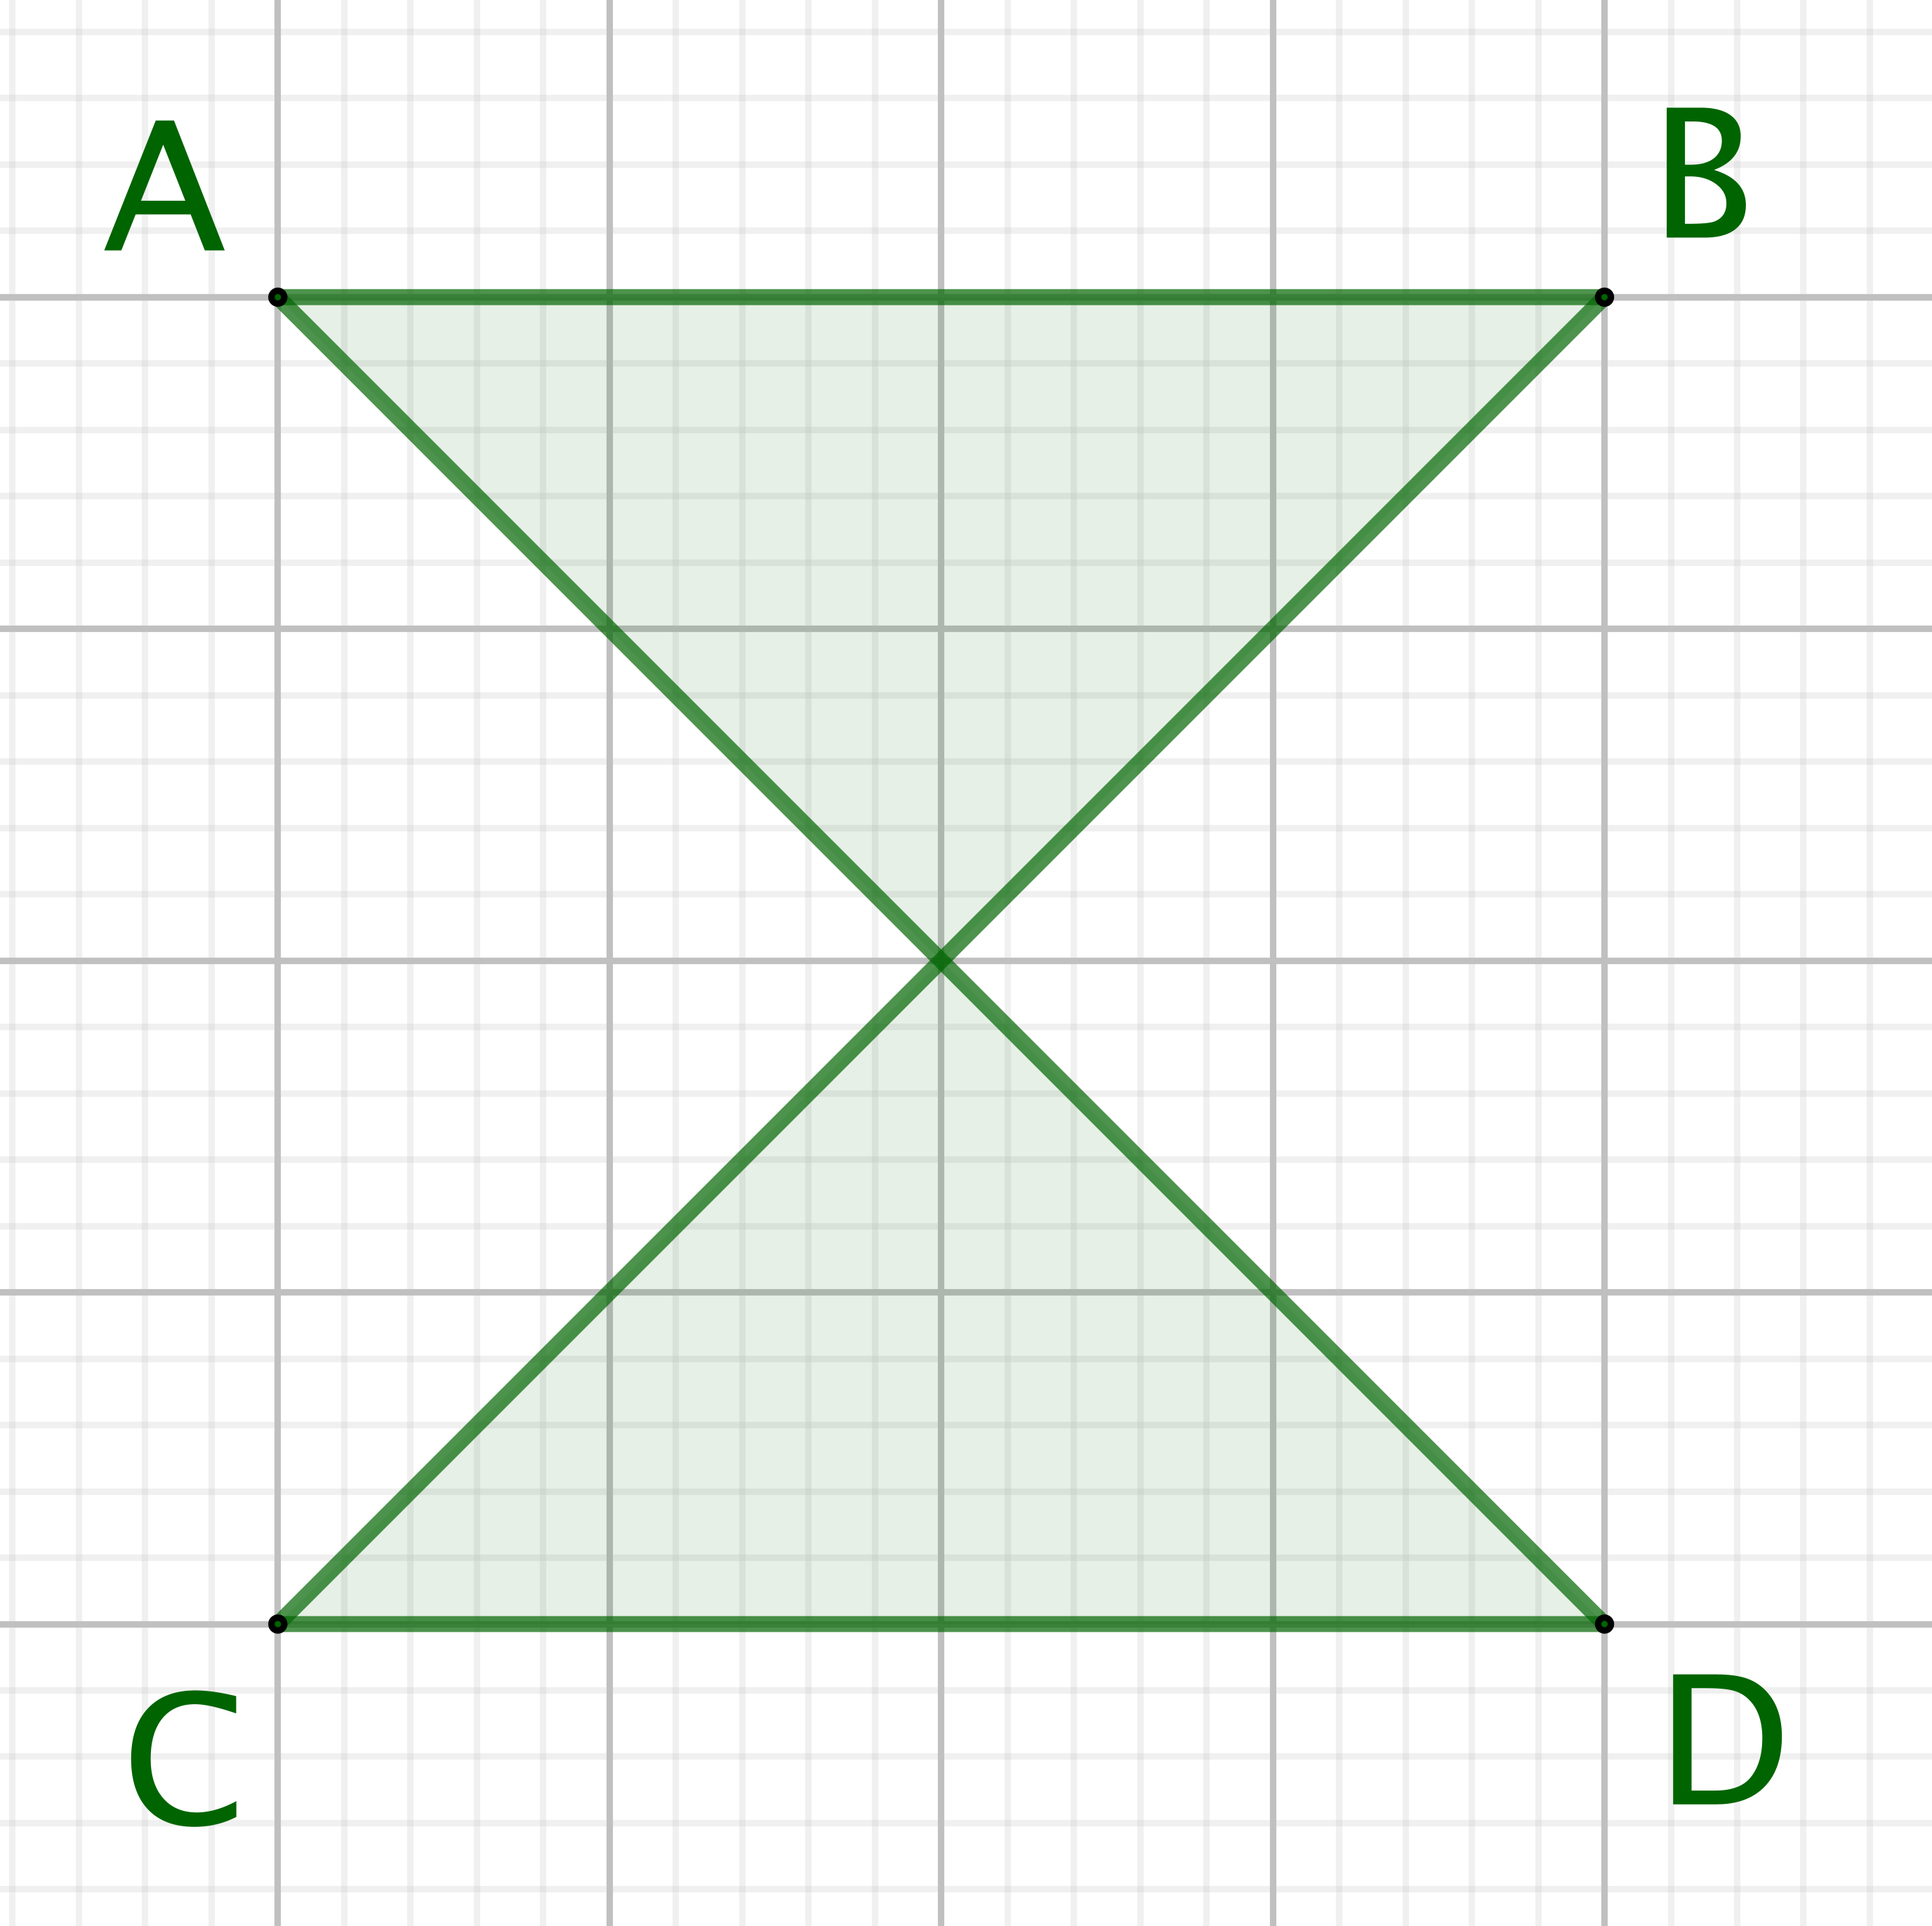
\includegraphics[scale=.4]{content/polygon/sufficient-cond/alg-surf-anti-para.png}
\end{center}

	
% ----------------------- %


\begin{fact}
	Soit $\setproba{L} = A_1 A_2 \cdots A_n$ une \nline, et posons $A_{n+1} = A_n$.
	La fonction qui à un point $\Omega$ du plan associe 
	$\mu_{1 \to n}^\Omega (\setproba{L}) = \dsum_{i=1}^{n+1} \det \big( \vect{\Omega A_i} , \vect{\Omega A_{i+1}} \big)$ est indépendante du point $\Omega$.
	Dans la suite, cette quantité indépendante de $\Omega$ sera notée $\mu_{1 \to n} (\setproba{L})$.
\end{fact}


\begin{proof}
\end{proof}
	
	
% ----------------------- %


\begin{fact} \label{nline-shift-inva}
	Soit $\setproba{L} = A_1 A_2 \cdots A_n$ une \nline, et posons $A_{i + kn} = A_i$ pour $(i;k) \in \ZintervalC{1}{n} \times \NN$ afin de pouvoir définir aisément $\mu_{j \to n+j-1} (\setproba{L})$ pour $j \in \ZintervalC{1}{n}$.
	Dès lors, pour $j \in \ZintervalC{1}{n}$, nous avons
	$\mu_{1 \to n} (\setproba{L}) = \mu_{j \to n+j-1} (\setproba{L})$.
	Dans la suite, cette quantité commune sera notée $\mu_1^n (\setproba{L})$.
\end{fact}


\begin{proof}
\end{proof}
	
	
% ----------------------- %


\begin{fact} \label{nline-rota-inva}
	Soient 
	$\setproba{L} = A_1 A_2 \cdots A_n$ une \nline, et 
	$\setproba{L}^{\mathrm{op}} = A_n A_{n-1} \cdots A_1$ la \nline\ obtenue via un parcours inversé à partir de $A_n$, 
	Posant $B_i = A_{n + 1 - i}$, nous avons $\setproba{L}^{\mathrm{op}} = B_1 B_2 \cdots B_n$ qui permet de considérer $\mu_1^n (\setproba{L}^{\mathrm{op}})$.
	Dès lors, nous avons
	$\mu_1^n (\setproba{L}) = {} - \mu_1^n (\setproba{L}^{\mathrm{op}})$.
\end{fact}


\begin{proof}
\end{proof}
	
	
% ----------------------- %


\begin{fact}
	Soit 
	$\setproba{L} = A_1 A_2 \cdots A_n$ une \nline.
	La quantité $\abs{\mu_1^n (\setproba{L})}$ ne dépend ni du sens de parcours de de $\setproba{L}$,%
	\footnote{
		Le lecteur pardonnera cet abus de langage.
	}
	ni du point de départ choisi.
	Elle sera notée $\garea{\setproba{L}}$, et nommée \og \emph{aire généralisée} \fg\ de la \nline\ $\setproba{L}$.
\end{fact}


\begin{proof}
	C'est une synthèse des faits \ref{nline-shift-inva} et \ref{nline-rota-inva}.
\end{proof}
	
	
% ----------------------- %


\begin{fact}
	Pour tout \ngone\ $\setproba{P}$, nous avons: $\garea{\setproba{P}} = \area{\setproba{P}}$.
\end{fact}


\begin{proof}
\end{proof}


% ----------------------- %


\begin{fact} \label{suff-cond}
	Soit $n \in \NN_{\geq3}$ un naturel fixé.
	Considérons tous les \ngones\ de périmètre fixé. Parmi tous ces \ngones, il en existe au moins un d'aire maximale.
\end{fact}


\begin{proof}
	Le fait \ref{conv-poly} permet de considérer le problème de maximisation d'aire à périmètre fixé uniquement avec des \ngones\ convexes.
	Selon les faits \ref{iso-poly} et \ref{almost-reg-poly}, si parmi les \ngones\ convexes de périmètre fixé, il en existe un qui maximise l'aire, alors ce ne peut être que le \ngone\ régulier.
	Pour voir que cette condition nécessaire est suffisante, c
	%	
	\begin{itemize}
		\item On munit le plan d'un repère orthonormé $\pvaxes{O | i | j}$. 

		\item 
		XXX
		
		fermeture costaud, mais le côté birné !!!!
		
		pour fermeture, besoin d'accpeter les \kgones\ pour $k \in \ZintervalC{3}{n}$.
		
		Les \ngones\ convexes $A_1 A_2 \cdots A_n$ tels que $\perim{A_1 A_2 \cdots A_n} = p$ sont représentés en posant $A_1\coord{0 | 0}$, $A_2\coord{A_1 A_2 | 0}$, puis $A_k\coord{x_k | y_k}$ avec $y_k \geq 0$ pour $k \in \ZintervalC{3}{n}$. Un \ngone\ peut donc avoir $n$ représentations, mais peu importe.
		De plus, on accepte les \ngones\ dégénérés pour lesquels nous avons $x_B = 0$, $y_C = 0$ dans notre représentation.
		Nous notons alors $\setproba{G} \subset \RR^{2n}$ l'ensemble des triplets $\coord{x_B | x_C | y_C}$ ainsi obtenus.

		\item XXX
		
		Justifier que $\setproba{G}$ est fermé dans $\RR^{2n}$.






		\item De plus, $\setproba{G}$ est borné, car les coordonnées des sommets des \kgones\ considérés le sont.		
		Finalement, $\setproba{G}$ est un compact de $\RR^{2n}$.


		\item Notons $s: \setproba{G} \rightarrow \RRp$ la fonction \og \emph{aire} \fg\ des \ngones\ représentés. 
		Cette fonction est continue en les coordonnées des sommets, car elle peut être calculée comme suit pour un \ngone\ convexe $A_1 A_2 \cdots A_n$ quelconque.
		%
		\begin{enumerate}
			\item L'isobarycentre $G$ de $A_1 A_2 \cdots A_n$ possède des coordonnées affines en celles des points $A_1$, $A_2$, \dots\ , et $A_n$.

			\item Par convexité, l'aire de $A_1 A_2 \cdots A_n$ est égale à la somme de celles des triangles $G A_k A_{k+1}$ pour $k \in \ZintervalC{1}{n-1}$, et du triangle $G A_n  A_1$.

			\item Via le déterminant, il est immédiat de voir que les aires des triangles considérés sont des fonctions continues en les coordonnées des sommets.
		\end{enumerate}
		
		
		\item Finalement, par continuité et compacité, on sait que $s$ admet un maximum sur $\setproba{G}$, un tel maximum ne pouvant pas être atteint sur un \kgone\ dégénéré. That's all folks!
	\end{itemize}	
\end{proof}










% ----------------------- %


\begin{fact}
	Soit $n \in \NN_{\geq3}$ un naturel fixé.
	Considérons tous les \ngones\  de périmètre fixé. Parmi tous ces \ngones, un seul est d'aire maximale, c'est le \ngone\ régulier.
\end{fact}


\begin{proof}
    C'est une conséquence directe des faits \ref{nece-cond} et \ref{suff-cond}.
\end{proof}